\lhead[\thepage]{CAPÍTULO \thechapter. ANÁLISIS}
\chead[]{}
\rhead[WepSIM: Simulador de un procesador elemental con unidad de control microprogramada\leftmark]{\thepage}
\renewcommand{\headrulewidth}{0.5pt}

\lfoot[]{}
\cfoot[]{}
\rfoot[]{}
\renewcommand{\footrulewidth}{0pt}

%% This is an example first chapter.  You should put chapter/appendix that you
%% write into a separate file, and add a line \include{yourfilename} to
%% main.tex, where `yourfilename.tex' is the name of the chapter/appendix file.
%% You can process specific files by typing their names in at the 
%% \files=
%% prompt when you run the file main.tex through LaTeX.
\chapter{Análisis}
\label{ch:analysis}
\markboth{}{ANALYSIS}

El objetivo principal de este capítulo, es describir el proyecto mediante la obtención y especificación de los requisitos del simulador, que puede proporcionar información suficiente para un análisis detallado que, por lo tanto, puede servir para continuar diseñando e implementando (Capítulos \ref{ch:design}, \textit{\nameref{ch:design}}; y \ref{ch:implementation_and_deployment}, \textit{\nameref{ch:implementation_and_deployment}}) un software que cumpla con esos requisitos. 

Con el fin de obtener los requisitos del sistema, el tutor ha desempeñado el papel del cliente en diferentes reuniones, mientras que el estudiante ha desempeñado los roles de analista, diseñador, programador y \emph{tester}.

La Sección \ref{sec:project_description} resume brevemente la descripción del proyecto. La Sección \ref{sec:requirements} especifica los requisitos del sistema, empezando con los requisitos de usuario y finalizando con los requisitos funcionales y no-funcionales. La Sección \ref{sec:user_cases} especifica los caso de uso del sistema. Finalmente, la Sección \ref{sec:regulatory_framework} indica el conjunto de leyes y regulaciones para la gestión del software.  

\section{Descripción del proyecto}
\label{sec:project_description}

El objetivo de este proyecto es construir una herramienta que permita simular con realismo el comportamiento de un procesador basado en la arquitectura indicada por el el tutor del proyecto, de forma que sirva como única herramienta para los estudiantes a lo largo de la asignatura Estructura de Computadores.

Los simuladores actuales para la enseñanza de Estructura de Computadores, están focalizados a una función concreta, como puede ser la simulación de cachés, la simulación de código ensamblador o la simulación de microcódigo entre otros, pero a la hora de unificar todas estas funcionalidades en una única herramienta, existe un vacío que genera una pérdida de tiempo en el aprendizaje de cada herramienta y la no posibilidad de ver una simulación completa.

El reto al que se enfrente cualquier simulador educativo es el de ser capaz de simular fielmente el funcionamiento de un dispositivo, permitiendo al estudiante poder observar con el mayor detalle posible el comportamiento éste.

El sistema que se propone debe ser capaz de simular con realismo el comportamiento del procesador, permitiendo la definición del juego de instrucciones a utilizar para el posterior desarrollo de código ensamblador y su ejecución en el simulador con un alto nivel de detalle en cada uno de los ciclos de ejecución. De esta forma, los estudiantes podrán comprender fácilmente los contenidos teóricos expuestos en la asignatura y serán capaces de realizar todas las prácticas en una misma herramienta, pudiendo ver de forma incremental el desarrollo de software de bajo nivel sobre un procesador elemental.


\section{Requisitos}
\label{sec:requirements}

Esta sección proporciona una descripción detallada de los requisitos de la aplicación. Para la tarea de la especificación de requisitos, se han seguido las prácticas recomendadas por IEEE \cite{ieee1998}. De acuerdo con estas prácticas, una buena especificación debe abordar la funcionalidad del software, los problemas de rendimiento, las interfaces externas, otras características no funcionales y las limitaciones de diseño o implementación.
Además, la especificación de los requisitos debe ser:

\begin{itemize}

\item \textbf{Completa:} el documento refleja todos los requisitos de software importantes.

\item \textbf{Consistente:} los requisitos no deben generar conflictos entre sí.

\item \textbf{Correcta:} cada requisito debe ser cumplido por el software según las necesidades del usuario.

% every requirement is one that the software shall meet according to the user needs.

\item \textbf{Modificable:} la estructura de la especificación permite cambios en los requisitos de una manera simple, completa y consistente.

\item \textbf{Clasificación basada en la importancia y la estabilidad:} cada requisito debe indicar su importancia y su estabilidad.

\item \textbf{Trazable:} el origen de cada requisito es claro y se puede hacer referencia fácilmente en otras etapas.

\item \textbf{Inequívoco:} cada requisito tiene una sola interpretación.

\item \textbf{Verificable:} Cada requisito debe ser verificable, es decir, existe algún proceso para verificar que el software cumple con cada requisito.

\end{itemize}

A partir de los requisitos de los usuarios, que constituyen una referencia informal al comportamiento del producto que el cliente espera, derivamos los requisitos de software (en este caso, requisitos funcionales y no funcionales) que guiaron el proceso de diseño con información específica sobre la funcionalidad del sistema y otras características. Los requisitos recuperados se estructuraron de acuerdo con el siguiente esquema:

%Starting from the user requirements, which constitute an informal reference to the product p%erformance that the client expects, we derived the software requirements (in this case, functional r%equirements and non-functional requirements) that guided the design process with specific %nformation on the functionality of the system and other characteristics. The retrieved requirements %were structured according with the following schema:

\begin{itemize}
\item[1.] \textbf{Requisitos de usuario} 
	\begin{itemize}
		\item[(a)] \textbf{Capacidad:} el requisito describe la funcionalidad esperada del sistema como en casos de uso.
		\item[(b)] \textbf{Restricción:} el requisito especifica las restricciones o condiciones que el sistema debe cumplir.
	\end{itemize}	
\end{itemize}

\begin{itemize}
\item[2.] \textbf{Requisitos de software}
	\begin{itemize}
	\item[(a)] 	\textbf{Funcionales}
		\begin{itemize}
		\item[i.] 	\textbf{Funcional:} el requisito describe la funcionalidad básica y el propósito del sistema mientras se minimiza la ambigüedad.
		\item[ii.] 	\textbf{Inverso:} el requisito limita la funcionalidad de la aplicación para aclarar su alcance.
		\end{itemize}

	\item[(b)] 	\textbf{No-Funcionales}
		\begin{itemize}
		\item[i.] 	\textbf{Rendimiento:} el requisito se relaciona con el rendimiento mínimo requerido del sistema resultante.
		\item[ii.] 	\textbf{Interfaz:} el requisito está relacionado con la interfaz de usuario de la aplicación.
		\item[iii.] 	\textbf{Escalabilidad:} el requisito está relacionado con la capacidad del sistema para adaptarse a cargas de trabajo cada vez mayores.
		\item[iv.] 	\textbf{Plataforma:} el requisito especifica las plataformas subyacentes de software y hardware en las que funcionará el sistema.
		\end{itemize}			
	\end{itemize}
\end{itemize}

La Tabla \ref{tab:requirements_template} proporciona la plantilla utilizada para la especificación de requisitos. Es necesario tener en cuenta que para los requisitos del usuario, el formato de identificación será UR-XYY, donde X indica el subtipo de requisito: requisitos de capacidad (C) o restricciones (R). YY corresponde al número de requisito en su subcategoría. Para los requisitos de software, se utilizará el formato de identificación SR-X-YZZ, donde X indica si es un requisito funcional (F) o no funcional (NF), e Y representa su subcategoría: funcional (F), inversa (I) ), Rendimiento (P), interfaz (UI), escalabilidad (S) o plataforma (PL). ZZ corresponde al número de requisito en su subcategoría.

\begin{center}
\begin{table*}[htbp]
\centering
\caption{Plantilla para la especificación de requisitos.}
\begin{tabular}{@{}p{2.5cm} p{9cm}@{}} 
\toprule
\textbf{ID} 				& Requisito ID. \\
\midrule
\textbf{Nombre} 			& Nombre del requisito. \\
\midrule
\textbf{Tipo} 			& Indica la categoría en la que se colocaría el requisito de acuerdo con el esquema descrito anteriormente. \\
\midrule
\textbf{Origen} 			& Constituye la fuente del requisito. Puede ser el usuario, otro requisito u otros actores involucrados en el proyecto. \\
\midrule
\textbf{Prioridad}		& Indica la prioridad del requisito según su importancia. Un requisito puede ser identificado como \textit{esencial}, \textit{condicional} or \textit{opcional}. \\
\midrule
\textbf{Estabilidad} 		& Indica la variabilidad del requisito a través del proceso de desarrollo, definido como \textit{estable} or \textit{inestable}. \\
\midrule
\textbf{Descripción} 	& Explicación detallada del requisito. \\
\bottomrule
\end{tabular}
\label{tab:requirements_template}
\end{table*}
\end{center}

\clearpage
\subsection{Requisitos de usuario}
\label{sec:user_requirements}

Esta subsección especifica los requisitos de usuario.

\begin{center}
\begin{table*}[htbp]
\centering
\caption{Requisito de usuario UR-C01.}
\begin{tabular}{@{}p{2.5cm} p{9cm}@{}} 
\toprule
\textbf{ID} 				& UR-C01 \\
\midrule
\textbf{Nombre} 			& Simulación del modelo hardware propuesto\\
\midrule
\textbf{Tipo} 			& Capacidad \\
\midrule
\textbf{Origen} 			& Usuario \\
\midrule
\textbf{Prioridad}		& Esencial \\
\midrule
\textbf{Estabilidad} 		& Estable \\
\midrule
\textbf{Descripción} 	& La herramienta simulará el comportamiento de la arquitectura definida para la asignatura Estructura de Computadores. \\
\bottomrule
\end{tabular}
\label{tab:urc01}
\end{table*}
\end{center}

\begin{center}
\begin{table*}[htbp]
\centering
\caption{Requisito de usuario UR-C02.}
\begin{tabular}{@{}p{2.5cm} p{9cm}@{}} 
\toprule
\textbf{ID} 				& UR-C02 \\
\midrule
\textbf{Nombre} 			& Definición de juego de instrucciones del simulador \\
\midrule
\textbf{Tipo} 			& Capacidad \\
\midrule
\textbf{Origen} 			& Usuario \\
\midrule
\textbf{Prioridad}		& Esencial \\
\midrule
\textbf{Estabilidad} 		& Estable \\
\midrule
\textbf{Descripción} 	& La herramienta debe permitir la definición del juego de instrucciones a utilizar por el usuario siguiendo el formato especificado por el tutor. \\
\bottomrule
\end{tabular}
\label{tab:urc02}
\end{table*}
\end{center}

\begin{center}
\begin{table*}[htbp]
\centering
\caption{Requisito de usuario UR-C03.}
\begin{tabular}{@{}p{2.5cm} p{9cm}@{}} 
\toprule
\textbf{ID} 				& UR-C03 \\
\midrule
\textbf{Nombre} 			& Operaciones con el juego de instrucciones \\
\midrule
\textbf{Tipo} 			& Capacidad \\
\midrule
\textbf{Origen} 			& Usuario \\
\midrule
\textbf{Prioridad}		& Esencial \\
\midrule
\textbf{Estabilidad} 		& Estable \\
\midrule
\textbf{Descripción} 	& La herramienta debe permitir al usuario las siguientes operaciones con el juego de instrucciones: cargar desde fichero, exportar a un fichero y generar el firmware. \\
\bottomrule
\end{tabular}
\label{tab:urc03}
\end{table*}
\end{center}

\begin{center}
\begin{table*}[htbp]
\centering
\caption{Requisito de usuario UR-C04.}
\begin{tabular}{@{}p{2.5cm} p{9cm}@{}} 
\toprule
\textbf{ID} 				& UR-C04 \\
\midrule
\textbf{Nombre} 			& Definición de juego del código ensamblador \\
\midrule
\textbf{Tipo} 			& Capacidad \\
\midrule
\textbf{Origen} 			& Usuario \\
\midrule
\textbf{Prioridad}		& Esencial \\
\midrule
\textbf{Estabilidad} 		& Estable \\
\midrule
\textbf{Descripción} 	& La herramienta debe permitir la definición del código ensamblador a simular siguiendo el formato utilizado en la asignatura Estructura de Computadores y el juego de instrucciones cargado previamente. \\
\bottomrule
\end{tabular}
\label{tab:urc04}
\end{table*}
\end{center}

\begin{center}
\begin{table*}[htbp]
\centering
\caption{Requisito de usuario UR-C05.}
\begin{tabular}{@{}p{2.5cm} p{9cm}@{}} 
\toprule
\textbf{ID} 				& UR-C05 \\
\midrule
\textbf{Nombre} 			& Operaciones con el código ensamblador \\
\midrule
\textbf{Tipo} 			& Capacidad \\
\midrule
\textbf{Origen} 			& Usuario \\
\midrule
\textbf{Prioridad}		& Esencial \\
\midrule
\textbf{Estabilidad} 		& Estable \\
\midrule
\textbf{Descripción} 	& La herramienta debe permitir al usuario las siguientes operaciones con el código ensamblador: cargar desde fichero, exportar a un fichero y generar el binario asociado. \\
\bottomrule
\end{tabular}
\label{tab:urc05}
\end{table*}
\end{center}

\begin{center}
\begin{table*}[htbp]
\centering
\caption{Requisito de usuario UR-C06.}
\begin{tabular}{@{}p{2.5cm} p{9cm}@{}} 
\toprule
\textbf{ID} 				& UR-C06 \\
\midrule
\textbf{Nombre} 			& Tipos de simulación \\
\midrule
\textbf{Tipo} 			& Capacidad \\
\midrule
\textbf{Origen} 			& Usuario \\
\midrule
\textbf{Prioridad}		& Esencial \\
\midrule
\textbf{Estabilidad} 		& Estable \\
\midrule
\textbf{Descripción} 	& La herramienta debe permitir tres tipos diferentes de simulación: simulación ciclo a ciclo de reloj, simulación instrucción a instrucción y simulación completa del código.\\
\bottomrule
\end{tabular}
\label{tab:urc06}
\end{table*}
\end{center}

\begin{center}
\begin{table*}[htbp]
\centering
\caption{Requisito de usuario UR-C07.}
\begin{tabular}{@{}p{2.5cm} p{9cm}@{}} 
\toprule
\textbf{ID} 				& UR-C07 \\
\midrule
\textbf{Nombre} 			& Configuración de la velocidad de las simulaciones \\
\midrule
\textbf{Tipo} 			& Capacidad \\
\midrule
\textbf{Origen} 			& Usuario \\
\midrule
\textbf{Prioridad}		& Esencial \\
\midrule
\textbf{Estabilidad} 		& Estable \\
\midrule
\textbf{Descripción} 	& La herramienta debe permitir al usuario seleccionar la velocidad de la simulación. \\
\bottomrule
\end{tabular}
\label{tab:urc07}
\end{table*}
\end{center}

\begin{center}
\begin{table*}[htbp]
\centering
\caption{Requisito de usuario UR-C08.}
\begin{tabular}{@{}p{2.5cm} p{9cm}@{}} 
\toprule
\textbf{ID} 				& UR-C08 \\
\midrule
\textbf{Nombre} 			& Esquemas de la arquitectura \\
\midrule
\textbf{Tipo} 			& Capacidad \\
\midrule
\textbf{Origen} 			& Usuario \\
\midrule
\textbf{Prioridad}		& Esencial \\
\midrule
\textbf{Estabilidad} 		& Estable \\
\midrule
\textbf{Descripción} 	& La herramienta debe mostrar la arquitectura de la CPU y la Unidad de Control que forman el simulador. \\
\bottomrule
\end{tabular}
\label{tab:urc08}
\end{table*}
\end{center}

\begin{center}
\begin{table*}[htbp]
\centering
\caption{Requisito de usuario UR-C09.}
\begin{tabular}{@{}p{2.5cm} p{9cm}@{}} 
\toprule
\textbf{ID} 				& UR-C09 \\
\midrule
\textbf{Nombre} 			& Información a mostrar \\
\midrule
\textbf{Tipo} 			& Capacidad \\
\midrule
\textbf{Origen} 			& Usuario \\
\midrule
\textbf{Prioridad}		& Esencial \\
\midrule
\textbf{Estabilidad} 		& Estable \\
\midrule
\textbf{Descripción} 	& La herramienta debe mostrar al usuario la información del estado del simulador en cada paso de la simulación. \\
\bottomrule
\end{tabular}
\label{tab:urc09}
\end{table*}
\end{center}


\begin{center}
\begin{table*}[htbp]
\centering
\caption{Requisito de usuario UR-R01.}
\begin{tabular}{@{}p{2.5cm} p{9cm}@{}} 
\toprule
\textbf{ID} 				& UR-R01 \\
\midrule
\textbf{Nombre} 			& Multiplataforma\\
\midrule
\textbf{Tipo} 			& Restricción \\
\midrule
\textbf{Origen} 			& Usuario \\
\midrule
\textbf{Prioridad}		& Esencial \\
\midrule
\textbf{Estabilidad} 		& Estable \\
\midrule
\textbf{Descripción} 	& El simulador no debe ser instalado en el dispositivo del usuario. \\
\bottomrule
\end{tabular}
\label{tab:urr01}
\end{table*}
\end{center}

\begin{center}
\begin{table*}[htbp]
\centering
\caption{Requisito de usuario UR-R02.}
\begin{tabular}{@{}p{2.5cm} p{9cm}@{}} 
\toprule
\textbf{ID} 				& UR-R02 \\
\midrule
\textbf{Nombre} 			& Navegadores web \\
\midrule
\textbf{Tipo} 			& Restricción \\
\midrule
\textbf{Origen} 			& Usuario \\
\midrule
\textbf{Prioridad}		& Esencial \\
\midrule
\textbf{Estabilidad} 		& Estable \\
\midrule
\textbf{Descripción} 	& El simulador debe de funcionar en los siguiente navegadores web: Microsoft Edge 30+, Mozilla Firefox 45+, Google Chrome 50+ y Safari 10+. \\
\bottomrule
\end{tabular}
\label{tab:urr02}
\end{table*}
\end{center}

\begin{center}
\begin{table*}[htbp]
\centering
\caption{Requisito de usuario UR-R03.}
\begin{tabular}{@{}p{2.5cm} p{9cm}@{}} 
\toprule
\textbf{ID} 				& UR-R03 \\
\midrule
\textbf{Nombre} 			& Interfaz de usuario \\
\midrule
\textbf{Tipo} 			& Restricción \\
\midrule
\textbf{Origen} 			& Usuario \\
\midrule
\textbf{Prioridad}		& Esencial \\
\midrule
\textbf{Estabilidad} 		& Estable \\
\midrule
\textbf{Descripción} 	& La interfaz de usuario debe de ser compatible para uso en PCs y smartphones. \\
\bottomrule
\end{tabular}
\label{tab:urr03}
\end{table*}
\end{center}

\begin{center}
\begin{table*}[htbp]
\centering
\caption{Requisito de usuario UR-R04.}
\begin{tabular}{@{}p{2.5cm} p{9cm}@{}} 
\toprule
\textbf{ID} 				& UR-R04 \\
\midrule
\textbf{Nombre} 			& Tiempo por ciclo de reloj \\
\midrule
\textbf{Tipo} 			& Restricción \\
\midrule
\textbf{Origen} 			& Usuario \\
\midrule
\textbf{Prioridad}		& Esencial \\
\midrule
\textbf{Estabilidad} 		& Estable \\
\midrule
\textbf{Descripción} 	& El tiempo de ejecución en media de un ciclo de reloj del simulador no debe de sobrepasar 0,1 segundos. \\
\bottomrule
\end{tabular}
\label{tab:urr04}
\end{table*}
\end{center}

\begin{center}
\begin{table*}[htbp]
\centering
\caption{Requisito de usuario UR-R05.}
\begin{tabular}{@{}p{2.5cm} p{9cm}@{}} 
\toprule
\textbf{ID} 				& UR-R05 \\
\midrule
\textbf{Nombre} 			& Ejecución en local \\
\midrule
\textbf{Tipo} 			& Restricción \\
\midrule
\textbf{Origen} 			& Usuario \\
\midrule
\textbf{Prioridad}		& Esencial \\
\midrule
\textbf{Estabilidad} 		& Estable \\
\midrule
\textbf{Descripción} 	& Las simulaciones serán realizadas en el dispositivo del usuario, siendo únicamente necesario el servidor para el acceso a la herramienta. \\
\bottomrule
\end{tabular}
\label{tab:urr05}
\end{table*}
\end{center}

\begin{center}
\begin{table*}[htbp]
\centering
\caption{Requisito de usuario UR-R06.}
\begin{tabular}{@{}p{2.5cm} p{9cm}@{}} 
\toprule
\textbf{ID} 				& UR-R06 \\
\midrule
\textbf{Nombre} 			& Conexión a internet \\
\midrule
\textbf{Tipo} 			& Restricción \\
\midrule
\textbf{Origen} 			& Usuario \\
\midrule
\textbf{Prioridad}		& Esencial \\
\midrule
\textbf{Estabilidad} 		& Estable \\
\midrule
\textbf{Descripción} 	& La herramienta podrá ser ejecutada sin conexión a internet. \\
\bottomrule
\end{tabular}
\label{tab:urr06}
\end{table*}
\end{center}

\begin{center}
\begin{table*}[htbp]
\centering
\caption{Requisito de usuario UR-R07.}
\begin{tabular}{@{}p{2.5cm} p{9cm}@{}} 
\toprule
\textbf{ID} 				& UR-R07 \\
\midrule
\textbf{Nombre} 			& Tecnologías de desarrollo \\
\midrule
\textbf{Tipo} 			& Restricción \\
\midrule
\textbf{Origen} 			& Usuario \\
\midrule
\textbf{Prioridad}		& Esencial \\
\midrule
\textbf{Estabilidad} 		& Estable \\
\midrule
\textbf{Descripción} 	& El simulador debe de ser desarrollado mediante el lenguaje de programación HTML5. \\
\bottomrule
\end{tabular}
\label{tab:urr07}
\end{table*}
\end{center}

\subsection{Modelo de casos de uso}
\label{sec:user_cases}

Un caso de uso representa un uso típico que realizará alguno de los futuros usuarios del sistema desarrollado. El diagrama que se muestra a continuación representa los casos de uso de un usuario que utilice esta herramienta desarrollada. Se ha partido el diagrama en dos para hacerlo mucho más legible. A continuación, se muestra la primera parte del diagrama (Figura \ref{fig:user_cases1}). En la página siguiente se muestra la segunda parte (Figura \ref{fig:user_cases2}).

\begin{figure}[htbp]
 	\centering
 	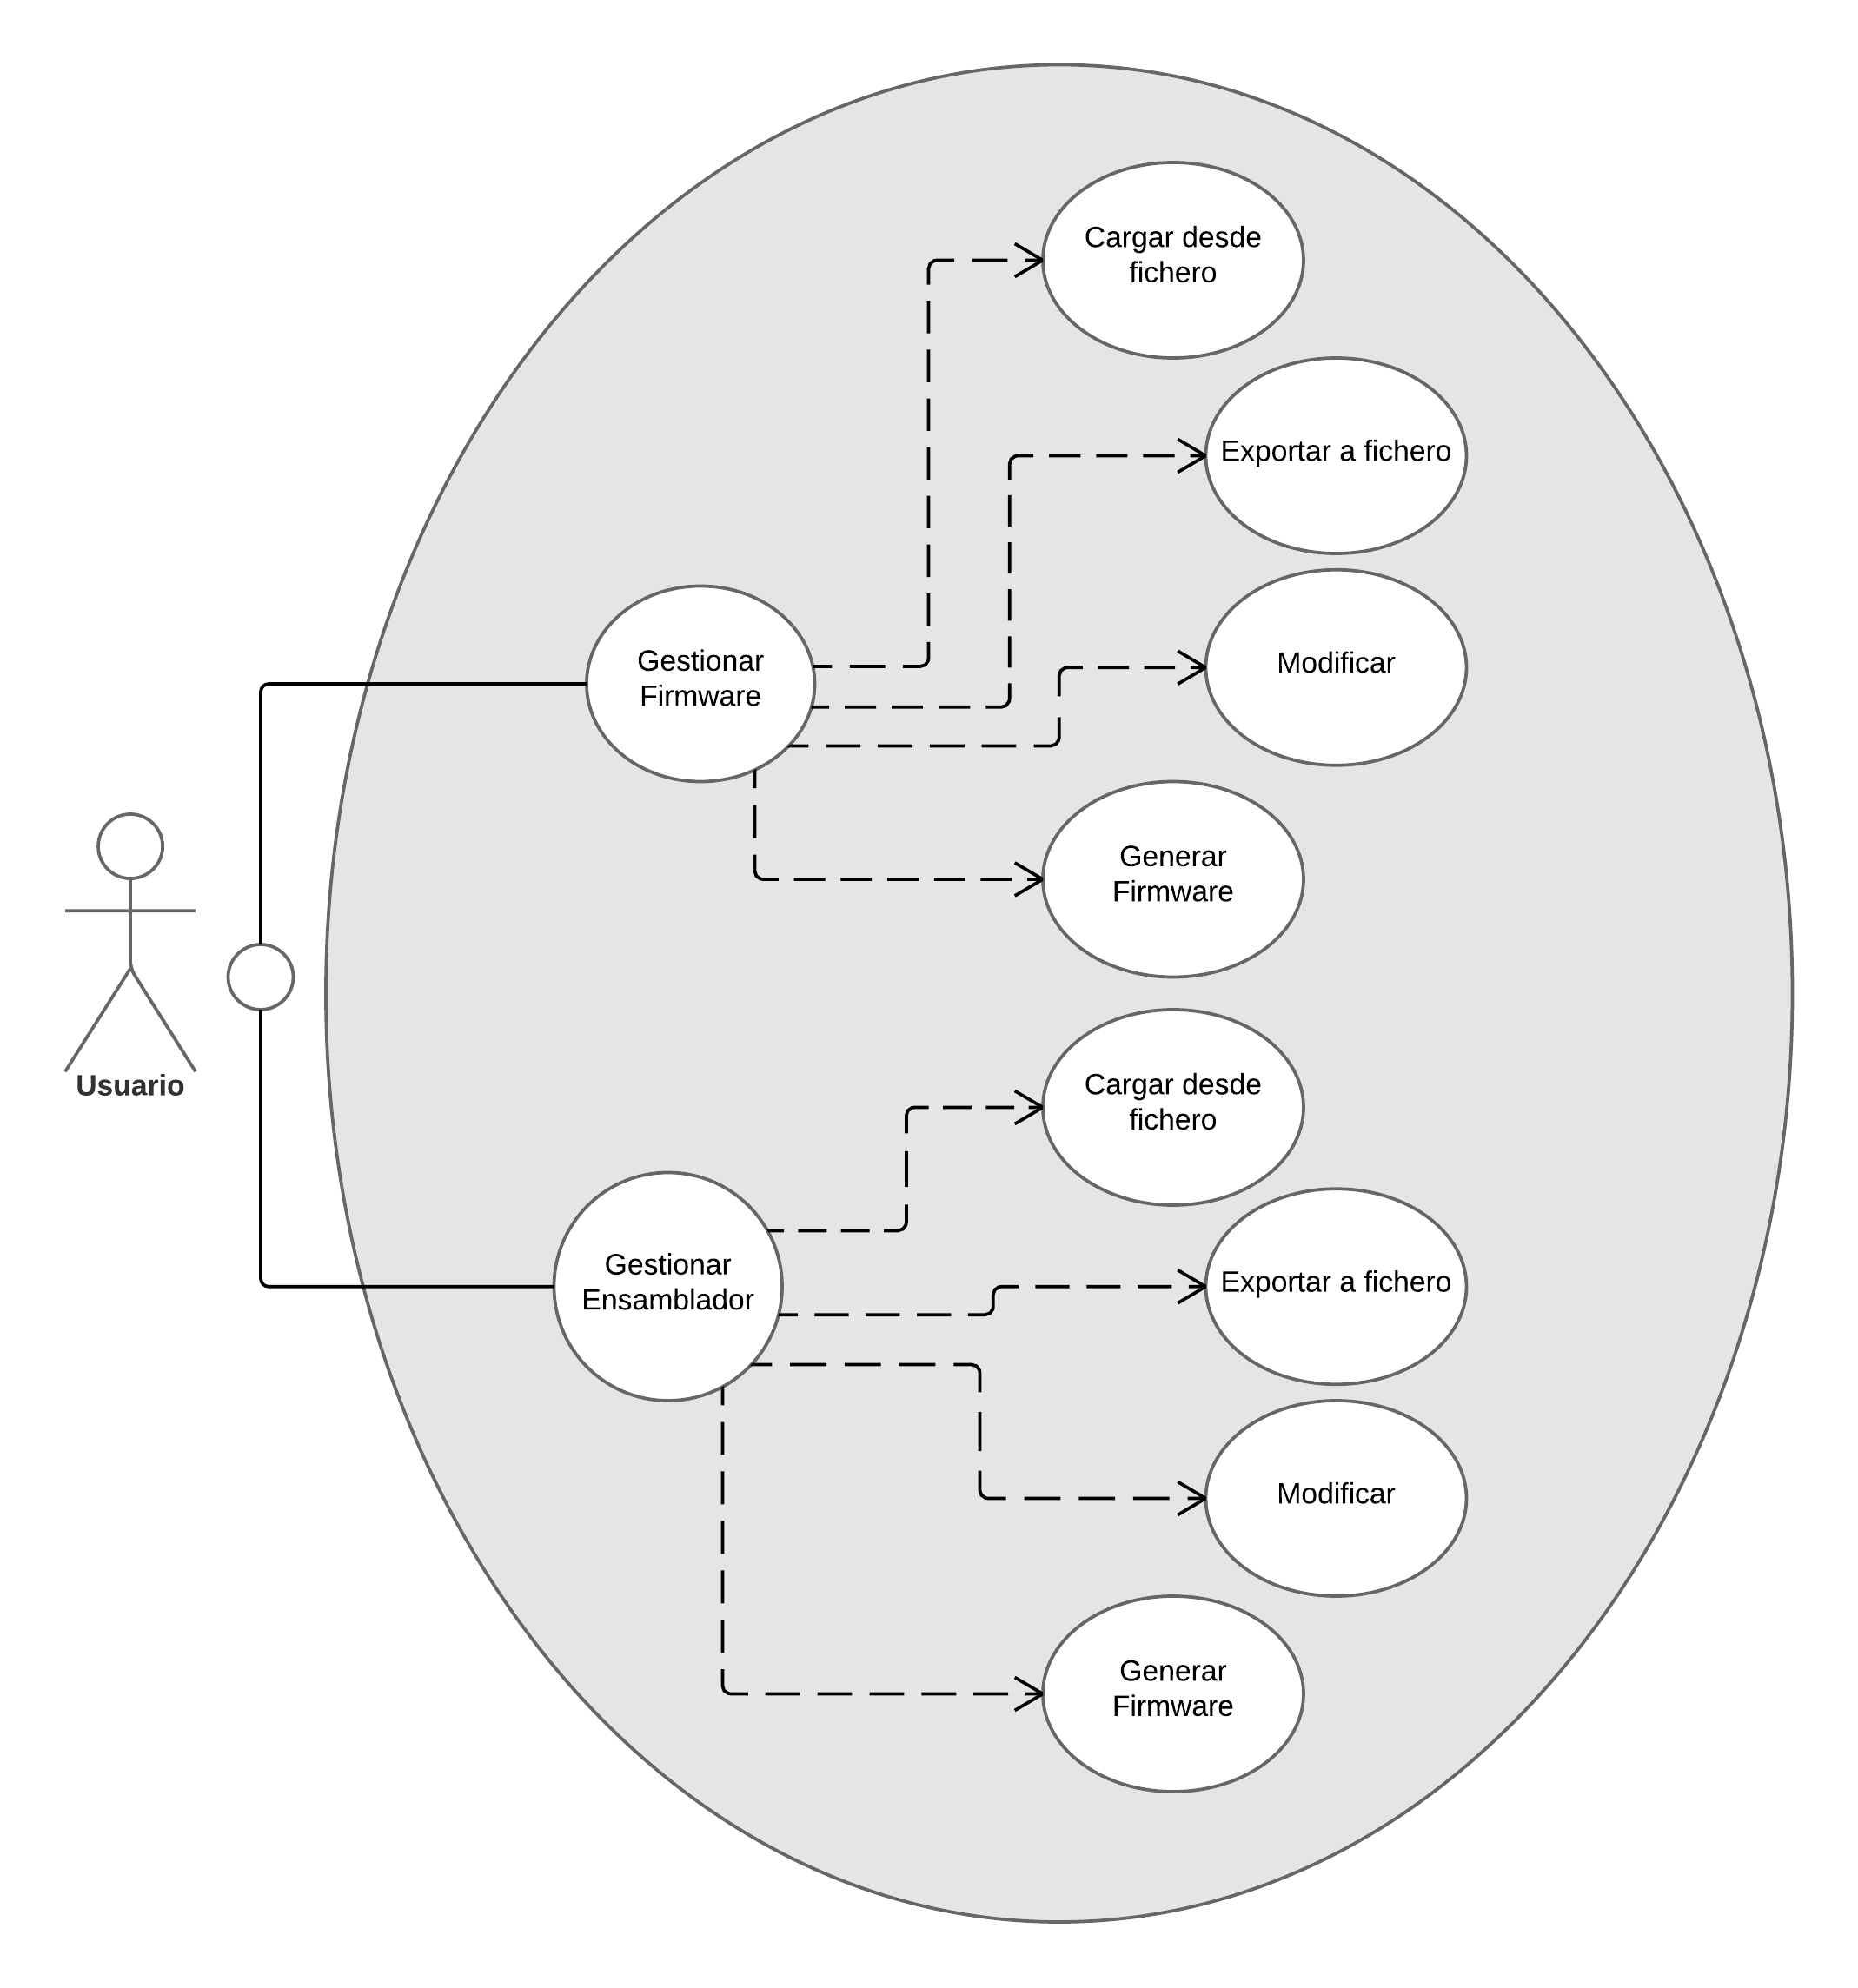
\includegraphics[width=14cm]{figures/user_cases_1}
 	\caption{Diagrama modelo casos de uso 1.}
	\label{fig:user_cases1}
\end{figure}

\vspace{20 mm}

\begin{figure}[htbp]
 	\centering
 	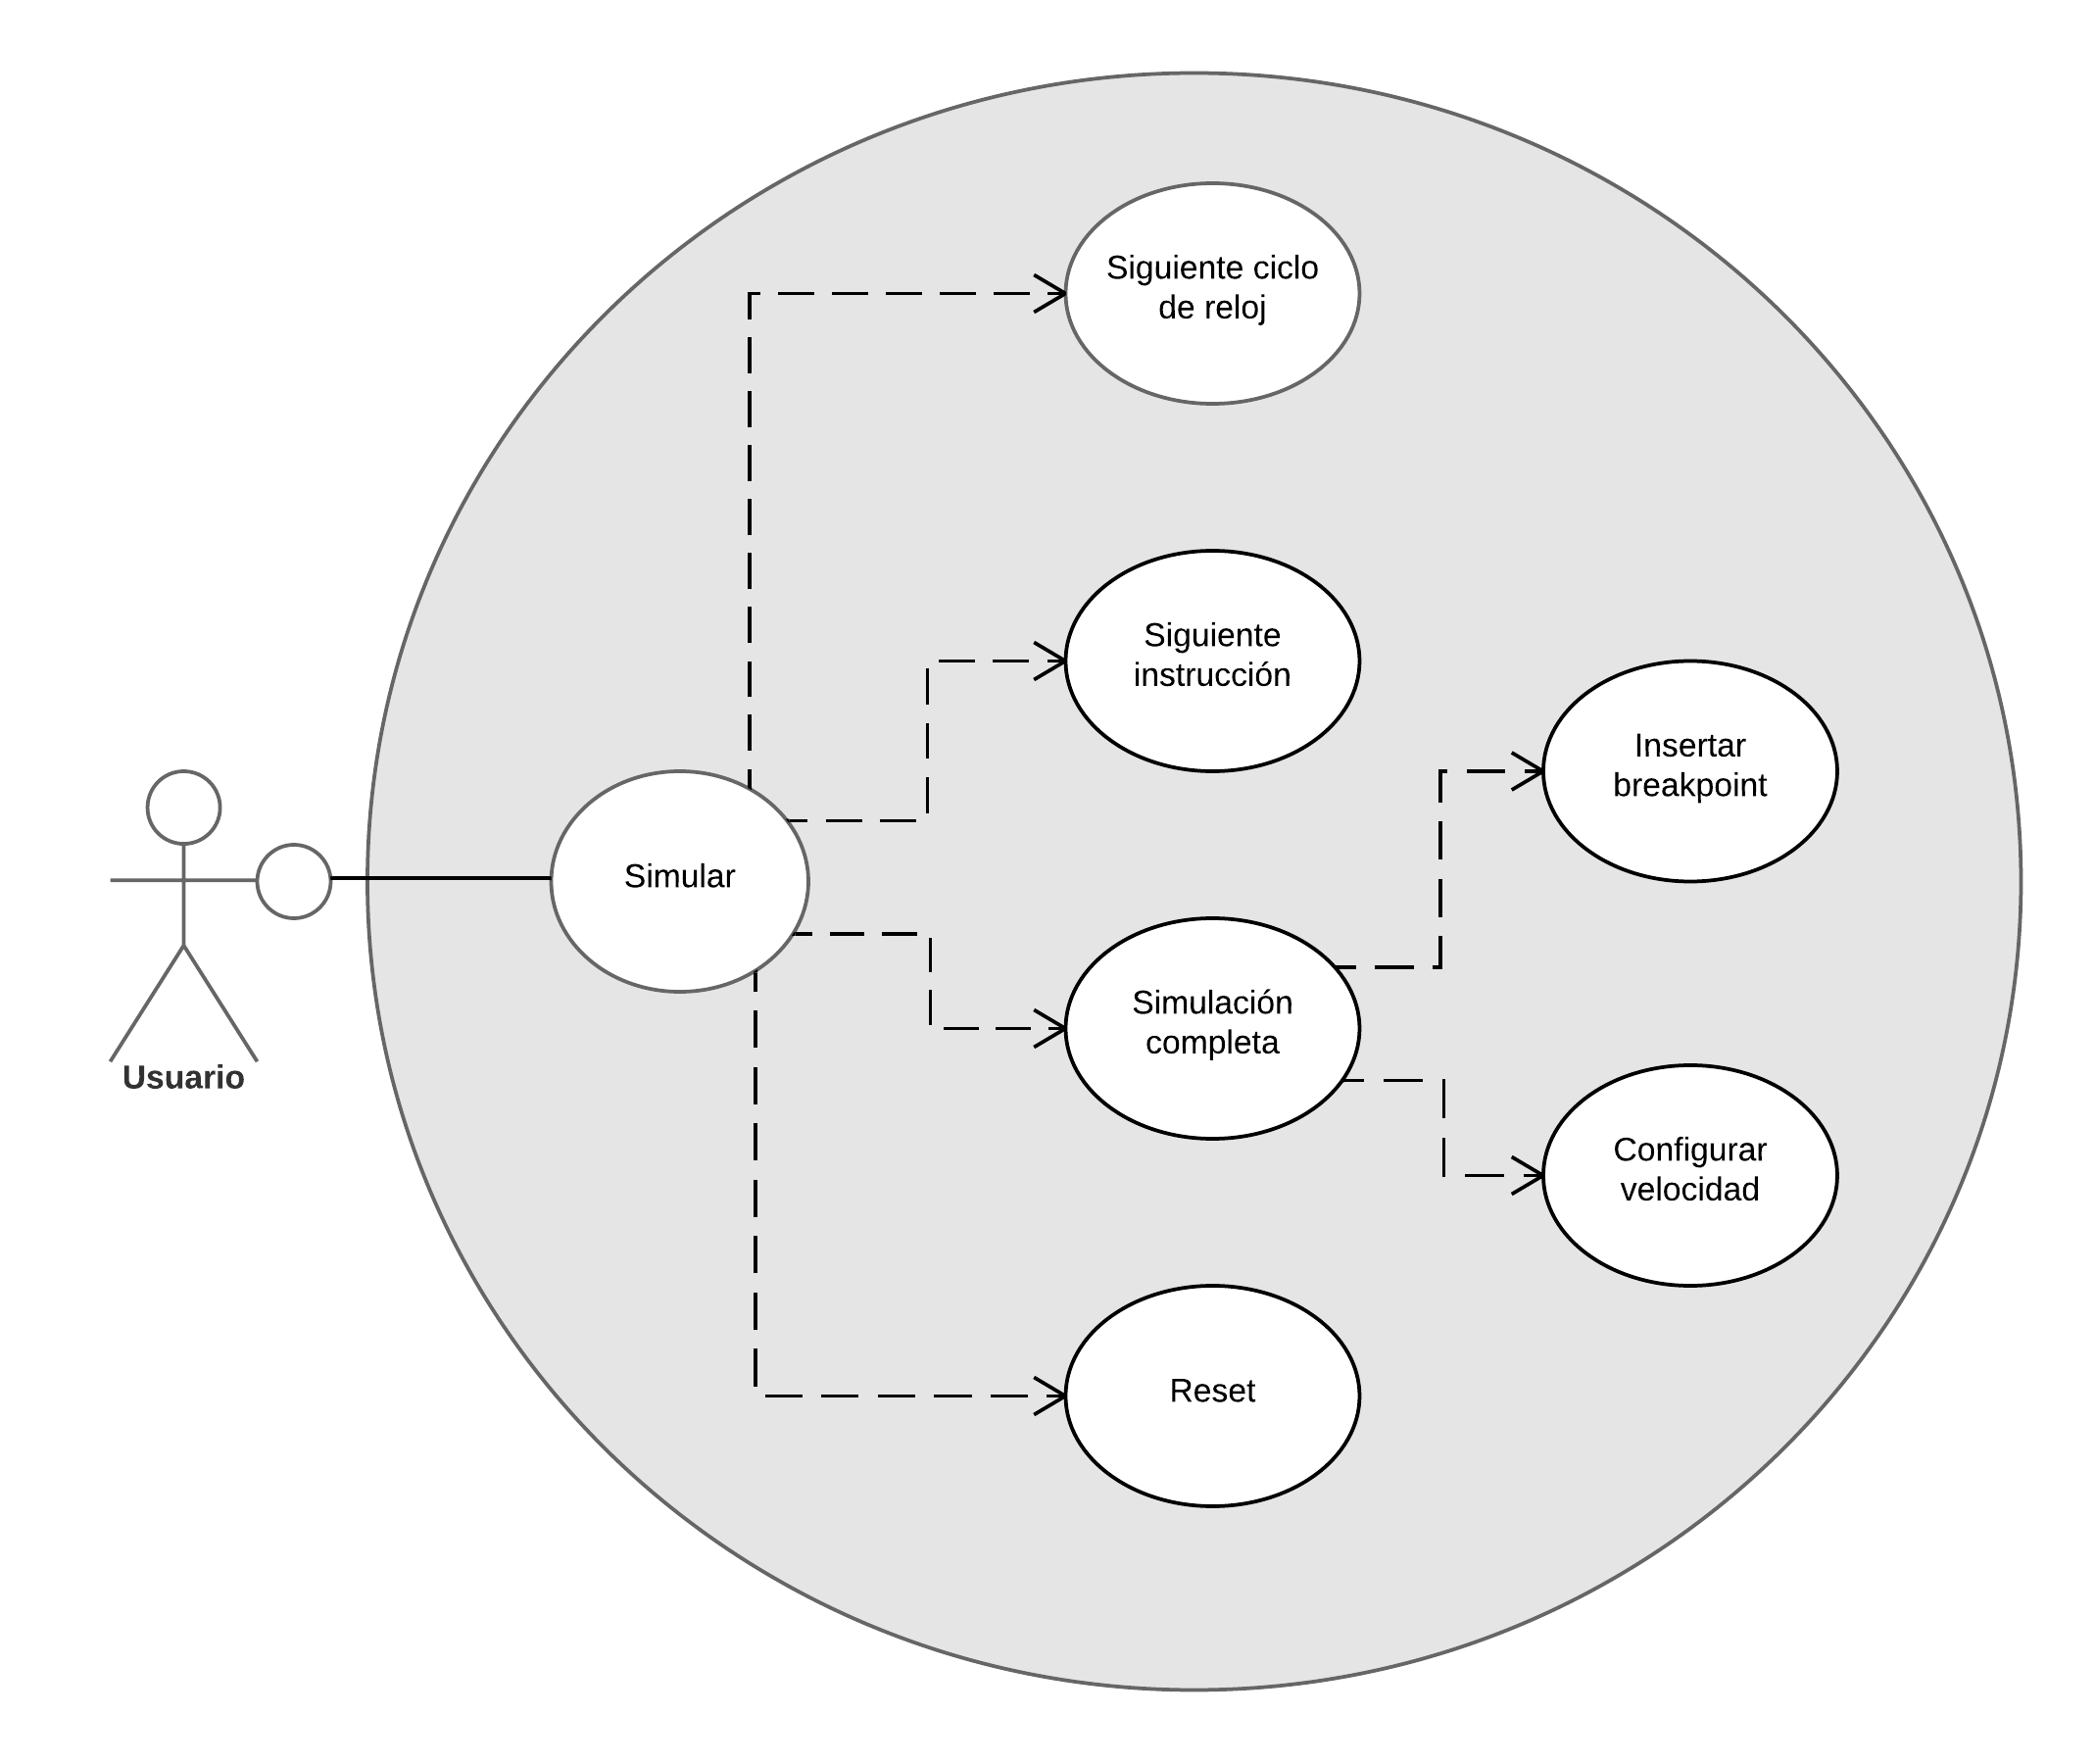
\includegraphics[width=15cm]{figures/user_cases_2}
 	\caption{Diagrama modelo casos de uso 2.}
	\label{fig:user_cases2}
\end{figure}

Para realizar la especificación clara, completa y detallada de cada uno de los casos de uso recogidos en el diagrama anterior se utilizará una tabla donde se recogerán los siguientes campos de información.

\begin{center}
\begin{table*}[htbp]
\centering
\caption{Plantilla de caso de uso.}
\begin{tabular}{@{}p{2.5cm} p{9cm}@{}} 
\toprule
\textbf{ID}	& Caso de uso ID.  \\
\midrule
\textbf{Nombre} 		& Nombre del caso de uso.   \\
\midrule
\textbf{Actores} 		&	Describe el actor o los actores que intervienen en la realización del caso de uso.  \\
\midrule
\textbf{Objetivo} 	&	Describe textualmente el cometido concreto del caso de uso. 	 \\
\midrule
\textbf{Precondiciones}	&	Muestra el estado del sistema que debe darse para que se pueda realizar el caso de uso.   \\
\midrule
\textbf{Postcondiciones} 	&	Presenta el estado del sistema tras la realización del caso de uso.   \\
\midrule
\textbf{Escenario Básico} 	&  Especifica la secuencia de pasos principales que se efectúan para realizar el caso de uso. \\
\bottomrule
\end{tabular}
\label{tab:uc_template}
\end{table*}
\end{center}

La Tabla \ref{tab:uc_template} proporciona la plantilla utilizada para la especificación de casos de uso. Es necesario tener en cuenta que el formato de identificación será UC-XX, donde XX corresponde al número del caso de uso. 

A continuación, se exponen los casos de uso.

\begin{center}
\begin{table*}[htbp]
\centering
\caption{Caso de uso UC-01.}
\begin{tabular}{@{}p{2.5cm} p{9cm}@{}} 
\toprule
\textbf{ID}	& UC-01  \\
\midrule
\textbf{Nombre} 		& Cargar juego de instrucciones   \\
\midrule
\textbf{Actores} 		&	Usuario  \\
\midrule
\textbf{Objetivo} 	&	Cargar en la herramienta un nuevo juego de instrucciones desde un fichero que indica el usuario. 	 \\
\midrule
\textbf{Precondiciones}	&	Ninguna.   \\
\midrule
\textbf{Postcondiciones} 	&	El juego de instrucciones se carga en la herramienta, mostrándose en el editor de texto correspondiente al firmware.   \\
\midrule
\textbf{Escenario Básico} 	&  \begin{itemize}
\item El usuario selecciona la pestaña firmware.
\item Pulsa el botón cargar firmware.
\item Selecciona el fichero deseado y acepta.
\end{itemize} \\
\bottomrule
\end{tabular}
\label{tab:uc01}
\end{table*}
\end{center}


\begin{center}
\begin{table*}[htbp]
\centering
\caption{Caso de uso UC-02}
\begin{tabular}{@{}p{2.5cm} p{9cm}@{}} 
\toprule
\textbf{ID}	& UC-02  \\
\midrule
\textbf{Nombre} 		& Exportar juego de instrucciones   \\
\midrule
\textbf{Actores} 		&	Usuario  \\
\midrule
\textbf{Objetivo} 	&	Exportar a un fichero el juego de instrucciones cargado en la memoria de control. 	 \\
\midrule
\textbf{Precondiciones}	&	La memoria de control ha sido generada.   \\
\midrule
\textbf{Postcondiciones} 	& Se genera un fichero en el dispositivo del usuario con el juego de instrucciones cargado previamente en la memoria de control.   \\
\midrule
\textbf{Escenario Básico} 	&  \begin{itemize}
\item El usuario selecciona la pestaña firmware.
\item Pulsa el botón guardar firmware.
\item Selecciona el nombre de fichero deseado y acepta.
\end{itemize} \\
\bottomrule
\end{tabular}
\label{tab:uc02}
\end{table*}
\end{center}

\begin{center}
\begin{table*}[htbp]
\centering
\caption{Caso de uso UC-03.}
\begin{tabular}{@{}p{2.5cm} p{9cm}@{}} 
\toprule
\textbf{ID}	& UC-03  \\
\midrule
\textbf{Nombre} 		& Modificar juego de instrucciones   \\
\midrule
\textbf{Actores} 		&	Usuario  \\
\midrule
\textbf{Objetivo} 	&	Editar el juego de instrucciones desde la herramienta. 	 \\
\midrule
\textbf{Precondiciones}	&	Ninguna.   \\
\midrule
\textbf{Postcondiciones} 	& Las modificaciones realizadas por el usuario en el juego de instrucciones son mostradas en el editor de texto correspondiente al firmware.   \\
\midrule
\textbf{Escenario Básico} 	&  \begin{itemize}
\item El usuario selecciona la pestaña firmware.
\item Realiza las modificaciones deseadas en el editor de texto.
\end{itemize} \\
\bottomrule
\end{tabular}
\label{tab:uc03}
\end{table*}
\end{center}

\begin{center}
\begin{table*}[htbp]
\centering
\caption{Caso de uso UC-04.}
\begin{tabular}{@{}p{2.5cm} p{9cm}@{}} 
\toprule
\textbf{ID}	& UC-04  \\
\midrule
\textbf{Nombre} 		& Generar firmware   \\
\midrule
\textbf{Actores} 		&	Usuario  \\
\midrule
\textbf{Objetivo} 	&	Generar la memoria de control a partir del juego de instrucciones definido en la herramienta. 	 \\
\midrule
\textbf{Precondiciones}	&	El juego de instrucciones debe estar definido en la herramienta.   \\
\midrule
\textbf{Postcondiciones} 	& Se genera la memoria de control asociada al juego de instrucciones definido por el usuario.   \\
\midrule
\textbf{Escenario Básico} 	&  \begin{itemize}
\item El usuario selecciona la pestaña firmware.
\item Define el juego de instrucciones deseado en la herramienta.
\item Pulsa el botón generar firmware.
\end{itemize} \\
\bottomrule
\end{tabular}
\label{tab:uc04}
\end{table*}
\end{center}

\begin{center}
\begin{table*}[htbp]
\centering
\caption{Caso de uso UC-05.}
\begin{tabular}{@{}p{2.5cm} p{9cm}@{}} 
\toprule
\textbf{ID}	& UC-05  \\
\midrule
\textbf{Nombre} 		& Cargar ensamblador   \\
\midrule
\textbf{Actores} 		&	Usuario  \\
\midrule
\textbf{Objetivo} 	&	Cargar en la herramienta un nuevo código ensamblador desde un fichero que indica el usuario. 	 \\
\midrule
\textbf{Precondiciones}	&	Ninguna.   \\
\midrule
\textbf{Postcondiciones} 	& El código ensamblador se carga en la herramienta, mostrándose en el editor de texto correspondiente al ensamblador.   \\
\midrule
\textbf{Escenario Básico} 	&  \begin{itemize}
\item El usuario selecciona la pestaña ensamblador.
\item Pulsa el botón cargar ensamblador.
\item Selecciona el fichero deseado y acepta.
\end{itemize} \\
\bottomrule
\end{tabular}
\label{tab:uc05}
\end{table*}
\end{center}

\begin{center}
\begin{table*}[htbp]
\centering
\caption{Caso de uso UC-06.}
\begin{tabular}{@{}p{2.5cm} p{9cm}@{}} 
\toprule
\textbf{ID}	& UC-06  \\
\midrule
\textbf{Nombre} 		& Exportar ensamblador   \\
\midrule
\textbf{Actores} 		&	Usuario  \\
\midrule
\textbf{Objetivo} 	&	Exportar a un fichero el código ensamblador cargado para la simulación. 	 \\
\midrule
\textbf{Precondiciones}	&	El código ensamblador ha sido cargado en el simulador.   \\
\midrule
\textbf{Postcondiciones} 	& Se genera un fichero en el dispositivo del usuario con el código ensamblador cargado previamente en el simulador.   \\
\midrule
\textbf{Escenario Básico} 	&  \begin{itemize}
\item El usuario selecciona la pestaña ensamblador.
\item Pulsa el botón guardar ensamblador.
\item Selecciona el nombre de fichero deseado y acepta.
\end{itemize} \\
\bottomrule
\end{tabular}
\label{tab:uc06}
\end{table*}
\end{center}

\begin{center}
\begin{table*}[htbp]
\centering
\caption{Caso de uso UC-07.}
\begin{tabular}{@{}p{2.5cm} p{9cm}@{}} 
\toprule
\textbf{ID}	& UC-07  \\
\midrule
\textbf{Nombre} 		& Modificar ensamblador   \\
\midrule
\textbf{Actores} 		&	Usuario  \\
\midrule
\textbf{Objetivo} 	&	Editar el código ensamblador desde la herramienta. 	 \\
\midrule
\textbf{Precondiciones}	&	Ninguna.   \\
\midrule
\textbf{Postcondiciones} 	& Las modificaciones realizadas por el usuario en el juego de instrucciones son mostradas en el editor de texto correspondiente al firmware.   \\
\midrule
\textbf{Escenario Básico} 	&  \begin{itemize}
\item El usuario selecciona la pestaña ensamblador.
\item Realiza las modificaciones deseadas en el editor de texto.
\end{itemize} \\
\bottomrule
\end{tabular}
\label{tab:uc07}
\end{table*}
\end{center}

\begin{center}
\begin{table*}[htbp]
\centering
\caption{Caso de uso UC-08.}
\begin{tabular}{@{}p{2.5cm} p{9cm}@{}} 
\toprule
\textbf{ID}	& UC-08  \\
\midrule
\textbf{Nombre} 		& Generar memoria principal   \\
\midrule
\textbf{Actores} 		&	Usuario  \\
\midrule
\textbf{Objetivo} 	&	Cargar el código ensamblador definido por el usuario en el simulador, generando el contenido de la memoria principal correspondiente al ensamblador. 	 \\
\midrule
\textbf{Precondiciones}	&	El código ensamblador debe estar definido en la herramienta.  \\
\midrule
\textbf{Postcondiciones} 	& Se genera la memoria principal asociada al código ensamblador definido por el usuario.   \\
\midrule
\textbf{Escenario Básico} 	&  \begin{itemize}
\item El usuario selecciona la pestaña ensamblador.
\item Define el código ensamblador deseado en la herramienta.
\item Pulsa el botón compilar.
\end{itemize} \\
\bottomrule
\end{tabular}
\label{tab:uc08}
\end{table*}
\end{center}

\begin{center}
\begin{table*}[htbp]
\centering
\caption{Caso de uso UC-09.}
\begin{tabular}{@{}p{2.5cm} p{9cm}@{}} 
\toprule
\textbf{ID}	& UC-09  \\
\midrule
\textbf{Nombre} 		& Siguiente ciclo de reloj   \\
\midrule
\textbf{Actores} 		&	Usuario  \\
\midrule
\textbf{Objetivo} 	&	Avanzar un ciclo de reloj en la simulación.	 \\
\midrule
\textbf{Precondiciones}	&	La memoria de control y la memoria principal deben de estar generadas.  \\
\midrule
\textbf{Postcondiciones} 	& La ejecución de la simulación avanza un ciclo de reloj, siendo modificado el estado del simulador.   \\
\midrule
\textbf{Escenario Básico} 	&  \begin{itemize}
\item El usuario selecciona la pestaña simulador.
\item Pulsa el botón siguiente micro-instrucción.
\end{itemize} \\
\bottomrule
\end{tabular}
\label{tab:uc09}
\end{table*}
\end{center}

\begin{center}
\begin{table*}[htbp]
\centering
\caption{Caso de uso UC-10.}
\begin{tabular}{@{}p{2.5cm} p{9cm}@{}} 
\toprule
\textbf{ID}	& UC-10  \\
\midrule
\textbf{Nombre} 		& Siguiente instrucción   \\
\midrule
\textbf{Actores} 		&	Usuario  \\
\midrule
\textbf{Objetivo} 	&	Avanzar una instrucción en la simulación.	 \\
\midrule
\textbf{Precondiciones}	&	La memoria de control y la memoria principal deben de estar generadas.  \\
\midrule
\textbf{Postcondiciones} 	& La ejecución de la simulación avanza una instrucción, siendo modificado el estado del simulador.   \\
\midrule
\textbf{Escenario Básico} 	&  \begin{itemize}
\item El usuario selecciona la pestaña simulador.
\item Pulsa el botón siguiente instrucción.
\end{itemize} \\
\bottomrule
\end{tabular}
\label{tab:uc10}
\end{table*}
\end{center}

\begin{center}
\begin{table*}[htbp]
\centering
\caption{Caso de uso UC-11.}
\begin{tabular}{@{}p{2.5cm} p{9cm}@{}} 
\toprule
\textbf{ID}	& UC-11  \\
\midrule
\textbf{Nombre} 		& Insertar breakpoint  \\
\midrule
\textbf{Actores} 		&	Usuario  \\
\midrule
\textbf{Objetivo} 	&	Insertar un punto de detención en una instrucción del código ensamblador a simular.	 \\
\midrule
\textbf{Precondiciones}	&	La memoria de control y la memoria principal deben de estar generadas.  \\
\midrule
\textbf{Postcondiciones} 	& Se añade un breakpoint en la simulación.   \\
\midrule
\textbf{Escenario Básico} 	&  \begin{itemize}
\item El usuario selecciona la pestaña simulador.
\item Selecciona la pestaña Assembly Debugger.
\item Pulsa sobre la instrucción en la que añadir el breakpoint.
\end{itemize} \\
\bottomrule
\end{tabular}
\label{tab:uc11}
\end{table*}
\end{center}

\begin{center}
\begin{table*}[htbp]
\centering
\caption{Caso de uso UC-12.}
\begin{tabular}{@{}p{2.5cm} p{9cm}@{}} 
\toprule
\textbf{ID}	& UC-12  \\
\midrule
\textbf{Nombre} 		& Configurar velocidad  \\
\midrule
\textbf{Actores} 		&	Usuario  \\
\midrule
\textbf{Objetivo} 	&	Configurar la velocidad de la simulación.	 \\
\midrule
\textbf{Precondiciones}	&	La memoria de control y la memoria principal deben de estar generadas.  \\
\midrule
\textbf{Postcondiciones} 	& Se modifica la velocidad de la simulación.   \\
\midrule
\textbf{Escenario Básico} 	&  \begin{itemize}
\item El usuario selecciona la pestaña simulador.
\item Modifica la velocidad mediante la barra deslizable de velocidad.
\end{itemize} \\
\bottomrule
\end{tabular}
\label{tab:uc12}
\end{table*}
\end{center}

\begin{center}
\begin{table*}[htbp]
\centering
\caption{Caso de uso UC-13.}
\begin{tabular}{@{}p{2.5cm} p{9cm}@{}} 
\toprule
\textbf{ID}	& UC-13  \\
\midrule
\textbf{Nombre} 		& Reinicio del simulador  \\
\midrule
\textbf{Actores} 		&	Usuario  \\
\midrule
\textbf{Objetivo} 	&	Reiniciar la simulación.	 \\
\midrule
\textbf{Precondiciones}	&	La memoria de control y la memoria principal deben de estar generadas.  \\
\midrule
\textbf{Postcondiciones} 	& El simulador queda reiniciado y preparado para el comienzo de la simulación.   \\
\midrule
\textbf{Escenario Básico} 	&  \begin{itemize}
\item El usuario selecciona la pestaña simulador.
\item Pulsa sobre el botón reset.
\end{itemize} \\
\bottomrule
\end{tabular}
\label{tab:uc13}
\end{table*}
\end{center}


\clearpage
\subsection{Requisitos funcionales}

Esta subsección especifica los requisitos funcionales.

\begin{center}
\begin{table*}[htbp]
\centering
\caption{Requisito funcional SR-F-F01.}
\begin{tabular}{@{}p{2.5cm} p{9cm}@{}} 
\toprule
\textbf{ID} 				& SR-F-F01 \\
\midrule
\textbf{Nombre} 			& Arquitectura de 32 bits \\
\midrule
\textbf{Tipo} 			& Funcional \\
\midrule
\textbf{Origen} 			& UR-C01 \\
\midrule
\textbf{Prioridad}		& Esencial \\
\midrule
\textbf{Estabilidad} 		& Estable \\
\midrule
\textbf{Descripción} 	& La herramienta debe simular una arquitectura de 32 bits, implicando un banco de 32 registros, memoria principal con tamaño de  $2^{32}$ bits y registros y buses de 32 bits. \\
\bottomrule
\end{tabular}
\label{tab:srff01}
\end{table*}
\end{center}

\begin{center}
\begin{table*}[htbp]
\centering
\caption{Requisito funcional SR-F-F02.}
\begin{tabular}{@{}p{2.5cm} p{9cm}@{}} 
\toprule
\textbf{ID} 				& SR-F-F02 \\
\midrule
\textbf{Nombre} 			& Unidad de control microprogramable \\
\midrule
\textbf{Tipo} 			& Funcional \\
\midrule
\textbf{Origen} 			& UR-C01 \\
\midrule
\textbf{Prioridad}		& Esencial \\
\midrule
\textbf{Estabilidad} 		& Estable \\
\midrule
\textbf{Descripción} 	& La unidad de control debe de ser microprogramable, con secuenciamiento implícito, saltos a nivel de microdirección y microsaltos condicionales. \\
\bottomrule
\end{tabular}
\label{tab:srff02}
\end{table*}
\end{center}

\begin{center}
\begin{table*}[htbp]
\centering
\caption{Requisito funcional SR-F-F03.}
\begin{tabular}{@{}p{2.5cm} p{9cm}@{}} 
\toprule
\textbf{ID} 				& SR-F-F03 \\
\midrule
\textbf{Nombre} 			& Datos en complemento a dos (\emph{Ca2}) \\
\midrule
\textbf{Tipo} 			& Funcional \\
\midrule
\textbf{Origen} 			& UR-C01 \\
\midrule
\textbf{Prioridad}		& Esencial \\
\midrule
\textbf{Estabilidad} 		& Estable \\
\midrule
\textbf{Descripción} 	& La herramienta operará con una ALU de números enteros en complemento a dos. \\
\bottomrule
\end{tabular}
\label{tab:srff03}
\end{table*}
\end{center}

\begin{center}
\begin{table*}[htbp]
\centering
\caption{Requisito funcional SR-F-F04.}
\begin{tabular}{@{}p{2.5cm} p{9cm}@{}} 
\toprule
\textbf{ID} 				& SR-F-F04 \\
\midrule
\textbf{Nombre} 			& Definición de juego de instrucciones \\
\midrule
\textbf{Tipo} 			& Funcional \\
\midrule
\textbf{Origen} 			& UR-C02 \\
\midrule
\textbf{Prioridad}		& Esencial \\
\midrule
\textbf{Estabilidad} 		& Estable \\
\midrule
\textbf{Descripción} 	& La herramienta debe permitir al usuario la definición del juego de instrucciones a utilizar.\\
\bottomrule
\end{tabular}
\label{tab:srff04}
\end{table*}
\end{center}

\begin{center}
\begin{table*}[htbp]
\centering
\caption{Requisito funcional SR-F-F05.}
\begin{tabular}{@{}p{2.5cm} p{9cm}@{}} 
\toprule
\textbf{ID} 				& SR-F-F05 \\
\midrule
\textbf{Nombre} 			& Formato del juego de instrucciones\\
\midrule
\textbf{Tipo} 			& Funcional \\
\midrule
\textbf{Origen} 			& UR-C02 \\
\midrule
\textbf{Prioridad}		& Esencial \\
\midrule
\textbf{Estabilidad} 		& Estable \\
\midrule
\textbf{Descripción} 	& El juego de instrucciones debe seguir el formato utilizado en la asignatura Estructura de Computadores, definiendo instrucciones del lenguaje ensamblador, su microcódigo asociado, nombrado de los registros y pseudoinstrucciones. \\
\bottomrule
\end{tabular}
\label{tab:srff05}
\end{table*}
\end{center}

\begin{center}
\begin{table*}[htbp]
\centering
\caption{Requisito funcional SR-F-F06.}
\begin{tabular}{@{}p{2.5cm} p{9cm}@{}} 
\toprule
\textbf{ID} 				& SR-F-F06 \\
\midrule
\textbf{Nombre} 			& Modificación del juego de instrucciones\\
\midrule
\textbf{Tipo} 			& Funcional \\
\midrule
\textbf{Origen} 			& UR-C03 \\
\midrule
\textbf{Prioridad}		& Esencial \\
\midrule
\textbf{Estabilidad} 		& Estable \\
\midrule
\textbf{Descripción} 	& La herramienta debe de permitir la modificación del juego de instrucciones a utilizar por el usuario. \\
\bottomrule
\end{tabular}
\label{tab:srff06}
\end{table*}
\end{center}

\begin{center}
\begin{table*}[htbp]
\centering
\caption{Requisito funcional SR-F-F07.}
\begin{tabular}{@{}p{2.5cm} p{9cm}@{}} 
\toprule
\textbf{ID} 				& SR-F-F07 \\
\midrule
\textbf{Nombre} 			& Carga de juego de instrucciones\\
\midrule
\textbf{Tipo} 			& Funcional \\
\midrule
\textbf{Origen} 			& UR-C03 \\
\midrule
\textbf{Prioridad}		& Esencial \\
\midrule
\textbf{Estabilidad} 		& Estable \\
\midrule
\textbf{Descripción} 	& La herramienta debe permitir la carga de un fichero que contenga el juego de instrucciones. \\
\bottomrule
\end{tabular}
\label{tab:srff07}
\end{table*}
\end{center}

\begin{center}
\begin{table*}[htbp]
\centering
\caption{Requisito funcional SR-F-F08.}
\begin{tabular}{@{}p{2.5cm} p{9cm}@{}} 
\toprule
\textbf{ID} 				& SR-F-F08 \\
\midrule
\textbf{Nombre} 			& Exportar juego de instrucciones\\
\midrule
\textbf{Tipo} 			& Funcional \\
\midrule
\textbf{Origen} 			& UR-C03 \\
\midrule
\textbf{Prioridad}		& Esencial \\
\midrule
\textbf{Estabilidad} 		& Estable \\
\midrule
\textbf{Descripción} 	& La herramienta debe permitir exportar el juego de instrucciones en un fichero. \\
\bottomrule
\end{tabular}
\label{tab:srff08}
\end{table*}
\end{center}

\begin{center}
\begin{table*}[htbp]
\centering
\caption{Requisito funcional SR-F-F09.}
\begin{tabular}{@{}p{2.5cm} p{9cm}@{}} 
\toprule
\textbf{ID} 				& SR-F-F09 \\
\midrule
\textbf{Nombre} 			& Generación firmware del simulador\\
\midrule
\textbf{Tipo} 			& Funcional \\
\midrule
\textbf{Origen} 			& UR-C03 \\
\midrule
\textbf{Prioridad}		& Esencial \\
\midrule
\textbf{Estabilidad} 		& Estable \\
\midrule
\textbf{Descripción} 	& La herramienta debe de generar el firmware simulador a partir del juego de instrucciones definido y cargado por el usuario. \\
\bottomrule
\end{tabular}
\label{tab:srff09}
\end{table*}
\end{center}

\begin{center}
\begin{table*}[htbp]
\centering
\caption{Requisito funcional SR-F-F10.}
\begin{tabular}{@{}p{2.5cm} p{9cm}@{}} 
\toprule
\textbf{ID} 				& SR-F-F10 \\
\midrule
\textbf{Nombre} 			& Definición del código ensamblador\\
\midrule
\textbf{Tipo} 			& Funcional \\
\midrule
\textbf{Origen} 			& UR-C04 \\
\midrule
\textbf{Prioridad}		& Esencial \\
\midrule
\textbf{Estabilidad} 		& Estable \\
\midrule
\textbf{Descripción} 	& La herramienta debe permitir al usuario la definición del código ensamblador a utilizar en la simulación. \\
\bottomrule
\end{tabular}
\label{tab:srff10}
\end{table*}
\end{center}

\begin{center}
\begin{table*}[htbp]
\centering
\caption{Requisito funcional SR-F-F11.}
\begin{tabular}{@{}p{2.5cm} p{9cm}@{}} 
\toprule
\textbf{ID} 				& SR-F-F11 \\
\midrule
\textbf{Nombre} 			& Formato del código ensamblador\\
\midrule
\textbf{Tipo} 			& Funcional \\
\midrule
\textbf{Origen} 			& UR-C04 \\
\midrule
\textbf{Prioridad}		& Esencial \\
\midrule
\textbf{Estabilidad} 		& Estable \\
\midrule
\textbf{Descripción} 	& El código ensamblador a simular debe de seguir el formato utilizado en la asignatura Estructura de Computadores, utilizando el lenguaje definido en el juego de instrucciones.\\
\bottomrule
\end{tabular}
\label{tab:srff11}
\end{table*}
\end{center}

\begin{center}
\begin{table*}[htbp]
\centering
\caption{Requisito funcional SR-F-F12.}
\begin{tabular}{@{}p{2.5cm} p{9cm}@{}} 
\toprule
\textbf{ID} 				& SR-F-F12 \\
\midrule
\textbf{Nombre} 			& Edición del código ensamblador\\
\midrule
\textbf{Tipo} 			& Funcional \\
\midrule
\textbf{Origen} 			& UR-C05 \\
\midrule
\textbf{Prioridad}		& Esencial \\
\midrule
\textbf{Estabilidad} 		& Estable \\
\midrule
\textbf{Descripción} 	& La herramienta debe permitir modificar el código ensamblador. \\
\bottomrule
\end{tabular}
\label{tab:srff12}
\end{table*}
\end{center}

\begin{center}
\begin{table*}[htbp]
\centering
\caption{Requisito funcional SR-F-F13.}
\begin{tabular}{@{}p{2.5cm} p{9cm}@{}} 
\toprule
\textbf{ID} 				& SR-F-F13 \\
\midrule
\textbf{Nombre} 			& Carga del código ensamblador\\
\midrule
\textbf{Tipo} 			& Funcional \\
\midrule
\textbf{Origen} 			& UR-C05 \\
\midrule
\textbf{Prioridad}		& Esencial \\
\midrule
\textbf{Estabilidad} 		& Estable \\
\midrule
\textbf{Descripción} 	& La herramienta debe permitir la carga de un fichero que contenga el código ensamblador. \\
\bottomrule
\end{tabular}
\label{tab:srff13}
\end{table*}
\end{center}

\begin{center}
\begin{table*}[htbp]
\centering
\caption{Requisito funcional SR-F-F14.}
\begin{tabular}{@{}p{2.5cm} p{9cm}@{}} 
\toprule
\textbf{ID} 				& SR-F-F14 \\
\midrule
\textbf{Nombre} 			& Exportar código ensamblador\\
\midrule
\textbf{Tipo} 			& Funcional \\
\midrule
\textbf{Origen} 			& UR-C05 \\
\midrule
\textbf{Prioridad}		& Esencial \\
\midrule
\textbf{Estabilidad} 		& Estable \\
\midrule
\textbf{Descripción} 	& La herramienta debe permitir exportar a un fichero el código ensamblador cargado en la herramienta. \\
\bottomrule
\end{tabular}
\label{tab:srff14}
\end{table*}
\end{center}

\begin{center}
\begin{table*}[htbp]
\centering
\caption{Requisito funcional SR-F-F15.}
\begin{tabular}{@{}p{2.5cm} p{9cm}@{}} 
\toprule
\textbf{ID} 				& SR-F-F15 \\
\midrule
\textbf{Nombre} 			& Generación ejecutable del código ensamblador\\
\midrule
\textbf{Tipo} 			& Funcional \\
\midrule
\textbf{Origen} 			& UR-C05 \\
\midrule
\textbf{Prioridad}		& Esencial \\
\midrule
\textbf{Estabilidad} 		& Estable \\
\midrule
\textbf{Descripción} 	& La herramienta debe de generar el binario ejecutable asociado al código ensamblador definido para la simulación. \\
\bottomrule
\end{tabular}
\label{tab:srff15}
\end{table*}
\end{center}

\begin{center}
\begin{table*}[htbp]
\centering
\caption{Requisito funcional SR-F-F16.}
\begin{tabular}{@{}p{2.5cm} p{9cm}@{}} 
\toprule
\textbf{ID} 				& SR-F-F16 \\
\midrule
\textbf{Nombre} 			& Simulación ciclo a ciclo de reloj\\
\midrule
\textbf{Tipo} 			& Funcional \\
\midrule
\textbf{Origen} 			& UR-C06 \\
\midrule
\textbf{Prioridad}		& Esencial \\
\midrule
\textbf{Estabilidad} 		& Estable \\
\midrule
\textbf{Descripción} 	& La herramienta debe de permitir la simulación ciclo a ciclo de reloj del código ensamblador cargado por el usuario. \\
\bottomrule
\end{tabular}
\label{tab:srff16}
\end{table*}
\end{center}

\begin{center}
\begin{table*}[htbp]
\centering
\caption{Requisito funcional SR-F-F17.}
\begin{tabular}{@{}p{2.5cm} p{9cm}@{}} 
\toprule
\textbf{ID} 				& SR-F-F17 \\
\midrule
\textbf{Nombre} 			& Simulación instrucción a instrucción\\
\midrule
\textbf{Tipo} 			& Funcional \\
\midrule
\textbf{Origen} 			& UR-C06 \\
\midrule
\textbf{Prioridad}		& Esencial \\
\midrule
\textbf{Estabilidad} 		& Estable \\
\midrule
\textbf{Descripción} 	& La herramienta debe de permitir la simulación instrucción a instrucción del código ensamblador cargado por el usuario. \\
\bottomrule
\end{tabular}
\label{tab:srff17}
\end{table*}
\end{center}

\begin{center}
\begin{table*}[htbp]
\centering
\caption{Requisito funcional SR-F-F18.}
\begin{tabular}{@{}p{2.5cm} p{9cm}@{}} 
\toprule
\textbf{ID} 				& SR-F-F18 \\
\midrule
\textbf{Nombre} 			& Simulación completa\\
\midrule
\textbf{Tipo} 			& Funcional \\
\midrule
\textbf{Origen} 			& UR-C06 \\
\midrule
\textbf{Prioridad}		& Esencial \\
\midrule
\textbf{Estabilidad} 		& Estable \\
\midrule
\textbf{Descripción} 	& La herramienta debe de permitir la simulación completa del código ensamblador cargado por el usuario. \\
\bottomrule
\end{tabular}
\label{tab:srff18}
\end{table*}
\end{center}

\begin{center}
\begin{table*}[htbp]
\centering
\caption{Requisito funcional SR-F-F19.}
\begin{tabular}{@{}p{2.5cm} p{9cm}@{}} 
\toprule
\textbf{ID} 				& SR-F-F19 \\
\midrule
\textbf{Nombre} 			& Velocidad de simulación\\
\midrule
\textbf{Tipo} 			& Funcional \\
\midrule
\textbf{Origen} 			& UR-C07 \\
\midrule
\textbf{Prioridad}		& Esencial \\
\midrule
\textbf{Estabilidad} 		& Estable \\
\midrule
\textbf{Descripción} 	& La herramienta debe de permitir al usuario elegir la velocidad de simulación del código ensamblador cargado. \\
\bottomrule
\end{tabular}
\label{tab:srff19}
\end{table*}
\end{center}

\begin{center}
\begin{table*}[htbp]
\centering
\caption{Requisito funcional SR-F-F20.}
\begin{tabular}{@{}p{2.5cm} p{9cm}@{}} 
\toprule
\textbf{ID} 				& SR-F-F20 \\
\midrule
\textbf{Nombre} 			& Esquema CPU\\
\midrule
\textbf{Tipo} 			& Funcional \\
\midrule
\textbf{Origen} 			& UR-C08 \\
\midrule
\textbf{Prioridad}		& Esencial \\
\midrule
\textbf{Estabilidad} 		& Estable \\
\midrule
\textbf{Descripción} 	& La herramienta debe de mostrar el esquema de la CPU del simulador, modificando el color de las señales activas y buses de datos actualizados en cada ciclo de reloj. \\
\bottomrule
\end{tabular}
\label{tab:srff20}
\end{table*}
\end{center}

\begin{center}
\begin{table*}[htbp]
\centering
\caption{Requisito funcional SR-F-F21.}
\begin{tabular}{@{}p{2.5cm} p{9cm}@{}} 
\toprule
\textbf{ID} 				& SR-F-F21 \\
\midrule
\textbf{Nombre} 			& Esquema unidad de control\\
\midrule
\textbf{Tipo} 			& Funcional \\
\midrule
\textbf{Origen} 			& UR-C08 \\
\midrule
\textbf{Prioridad}		& Esencial \\
\midrule
\textbf{Estabilidad} 		& Estable \\
\midrule
\textbf{Descripción} 	& La herramienta debe de mostrar el esquema de la unidad de control del simulador, modificando el color de las señales activas y buses de datos actualizados en cada ciclo de reloj. \\
\bottomrule
\end{tabular}
\label{tab:srff21}
\end{table*}
\end{center}

\begin{center}
\begin{table*}[htbp]
\centering
\caption{Requisito funcional SR-F-F22.}
\begin{tabular}{@{}p{2.5cm} p{9cm}@{}} 
\toprule
\textbf{ID} 				& SR-F-F22\\
\midrule
\textbf{Nombre} 			& Información de la simulación\\
\midrule
\textbf{Tipo} 			& Funcional \\
\midrule
\textbf{Origen} 			& UR-C09 \\
\midrule
\textbf{Prioridad}		& Esencial \\
\midrule
\textbf{Estabilidad} 		& Estable \\
\midrule
\textbf{Descripción} 	& La herramienta debe de mostrar durante la ejecución el estado de los registros del simulador. \\
\bottomrule
\end{tabular}
\label{tab:srff22}
\end{table*}
\end{center}

\subsection{Requisitos no-funcionales}

Esta subsección especifica los requisitos no-funcionales.

\begin{center}
\begin{table*}[htbp]
\centering
\caption{Requisito no-funcional SR-NF-PL01.}
\begin{tabular}{@{}p{2.5cm} p{9cm}@{}} 
\toprule
\textbf{ID} 				& SR-NF-PL01 \\
\midrule
\textbf{Nombre} 			&  Multiplataforma \\
\midrule
\textbf{Tipo} 			& Plataforma \\
\midrule
\textbf{Origen} 			& UR-R01 \\
\midrule
\textbf{Prioridad}		& Esencial \\
\midrule
\textbf{Estabilidad} 		& Estable \\
\midrule
\textbf{Descripción} 	& El simulador debe de ser diseñado como una aplicación web. \\
\bottomrule
\end{tabular}
\label{tab:srnfpl01}
\end{table*}
\end{center}

\begin{center}
\begin{table*}[htbp]
\centering
\caption{Requisito no-funcional SR-NF-PL02.}
\begin{tabular}{@{}p{2.5cm} p{9cm}@{}} 
\toprule
\textbf{ID} 				& SR-NF-PL02 \\
\midrule
\textbf{Nombre} 			& Navegadores web \\
\midrule
\textbf{Tipo} 			& Plataforma \\
\midrule
\textbf{Origen} 			& UR-R02 \\
\midrule
\textbf{Prioridad}		& Esencial \\
\midrule
\textbf{Estabilidad} 		& Estable \\
\midrule
\textbf{Descripción} 	& El simulador debe poder ser ejecutado en los navegadores: Microsoft Edge 30+, Mozilla Firefox 45+, Google Chrome 50+ y Safari 10+. \\
\bottomrule
\end{tabular}
\label{tab:srnfpl02}
\end{table*}
\end{center}

\begin{center}
\begin{table*}[htbp]
\centering
\caption{Requisito no-funcional SR-NF-PL03.}
\begin{tabular}{@{}p{2.5cm} p{9cm}@{}} 
\toprule
\textbf{ID} 				& SR-NF-PL03 \\
\midrule
\textbf{Nombre} 			& Plataforma de ejecución \\
\midrule
\textbf{Tipo} 			& Plataforma \\
\midrule
\textbf{Origen} 			& UR-R05 \\
\midrule
\textbf{Prioridad}		& Esencial \\
\midrule
\textbf{Estabilidad} 		& Estable \\
\midrule
\textbf{Descripción} 	& Las ejecuciones de la herramienta deben ser realizadas en el dispositivo del usuario. \\
\bottomrule
\end{tabular}
\label{tab:srnfpl03}
\end{table*}
\end{center}

\begin{center}
\begin{table*}[htbp]
\centering
\caption{Requisito no-funcional SR-NF-PL04.}
\begin{tabular}{@{}p{2.5cm} p{9cm}@{}} 
\toprule
\textbf{ID} 				& SR-NF-PL04 \\
\midrule
\textbf{Nombre} 			& Internet \\
\midrule
\textbf{Tipo} 			& Plataforma \\
\midrule
\textbf{Origen} 			& UR-R06 \\
\midrule
\textbf{Prioridad}		& Esencial \\
\midrule
\textbf{Estabilidad} 		& Estable \\
\midrule
\textbf{Descripción} 	& La herramienta podrá ser ejecutada sin conexión a internet. \\
\bottomrule
\end{tabular}
\label{tab:srnfpl04}
\end{table*}
\end{center}

\begin{center}
\begin{table*}[htbp]
\centering
\caption{Requisito no-funcional SR-NF-PL05.}
\begin{tabular}{@{}p{2.5cm} p{9cm}@{}} 
\toprule
\textbf{ID} 				& SR-NF-PL05 \\
\midrule
\textbf{Nombre} 			& Lenguaje de programación HTML5 \\
\midrule
\textbf{Tipo} 			& Plataforma \\
\midrule
\textbf{Origen} 			& UR-R07 \\
\midrule
\textbf{Prioridad}		& Esencial \\
\midrule
\textbf{Estabilidad} 		& Estable \\
\midrule
\textbf{Descripción} 	& La herramienta debe ser desarrollada en el lenguaje de programación HTML5 (HTML + CSS + JavaScript). \\
\bottomrule
\end{tabular}
\label{tab:srnfpl05}
\end{table*}
\end{center}

\begin{center}
\begin{table*}[htbp]
\centering
\caption{Requisito no-funcional SR-NF-UI01.}
\begin{tabular}{@{}p{2.5cm} p{9cm}@{}} 
\toprule
\textbf{ID} 				& SR-NF-UI01 \\
\midrule
\textbf{Nombre} 			& Interfaz de usuario \\
\midrule
\textbf{Tipo} 			& Interfaz \\
\midrule
\textbf{Origen} 			& UR-R03 \\
\midrule
\textbf{Prioridad}		& Esencial \\
\midrule
\textbf{Estabilidad} 		& Estable \\
\midrule
\textbf{Descripción} 	& La interfaz de usuario del simulador debe de ser compatible tanto con PCs como con plataformas móviles (tablets, smartphones, etc). \\
\bottomrule
\end{tabular}
\label{tab:srnfui01}
\end{table*}
\end{center}

\begin{center}
\begin{table*}[htbp]
\centering
\caption{Requisito no-funcional SR-NF-P01.}
\begin{tabular}{@{}p{2.5cm} p{9cm}@{}} 
\toprule
\textbf{ID} 				& SR-NF-P01 \\
\midrule
\textbf{Nombre} 			& Tiempo medio por ciclo de reloj \\
\midrule
\textbf{Tipo} 			& Rendimiento \\
\midrule
\textbf{Origen} 			& UR-R04 \\
\midrule
\textbf{Prioridad}		& Esencial \\
\midrule
\textbf{Estabilidad} 		& Estable \\
\midrule
\textbf{Descripción} 	& El tiempo medio de ejecución de un ciclo de reloj no debe exceder 0,1 segundos. \\
\bottomrule
\end{tabular}
\label{tab:srnfp01}
\end{table*}
\end{center}

La matriz de trazabilidad de entre requisitos de usuario y requisitos de software (Tabla \ref{tab:requirements_matrix}) determina que todos los requisitos de usuario quedan reflejados en los requisitos de software.

\begin{table}[htb]
\ra{1.3}
  \centering
  \caption{Matriz de trazabilidad de requisitos.}
  \begin{tabular}{@{}L{3cm}C{0.5cm}C{0.5cm}C{0.5cm}C{0.5cm}C{0.5cm}C{0.5cm}C{0.5cm}C{0.5cm}C{0.5cm}C{0.5cm}C{0.5cm}C{0.5cm}C{0.5cm}C{0.5cm}C{0.5cm}C{0.5cm}@{}}
    \toprule
     \thead{Requisitos} & \rothead{UR-C01} & \rothead{UR-C02} & \rothead{UR-C03} & \rothead{UR-C04}& \rothead{UR-C05} & \rothead{UR-C06} & \rothead{UR-C07} & \rothead{UR-C08} & \rothead{UR-C09} & \rothead{UR-R01} & \rothead{UR-R02} & \rothead{UR-R03} & \rothead{UR-R04} & \rothead{UR-R05} & \rothead{UR-R06} & \rothead{UR-R07} \\
    \midrule
    SR-F-F01 & \ding{51} & - & - & - & - & - & - & - & - & - & - & - & - & - & - & - \\
    SR-F-F02 & \ding{51} & - & - & - & - & - & - & - & - & - & - & - & - & - & - & - \\
    SR-F-F03 & \ding{51} & - & - & - & - & - & - & - & - & - & - & - & - & - & - & - \\
    SR-F-F04 & - & \ding{51} & - & - & - & - & - & - & - & - & - & - & - & - & - & - \\
    SR-F-F05 & - & \ding{51} & - & - & - & - & - & - & - & - & - & - & - & - & - & - \\
    SR-F-F06 & - & - & \ding{51} & - & - & - & - & - & - & - & - & - & - & - & - & - \\
    SR-F-F07 & - & - & \ding{51} & - & - & - & - & - & - & - & - & - & - & - & - & - \\
    SR-F-F08 & - & - & \ding{51} & - & - & - & - & - & - & - & - & - & - & - & - & - \\
    SR-F-F09 & - & - & \ding{51} & - & - & - & - & - & - & - & - & - & - & - & - & - \\
    SR-F-F10 & - & - & - & \ding{51} & - & - & - & - & - & - & - & - & - & - & - & - \\
    SR-F-F11 & - & - & - & \ding{51} & - & - & - & - & - & - & - & - & - & - & - & - \\
    SR-F-F12 & - & - & - & - & \ding{51} & - & - & - & - & - & - & - & - & - & - & - \\
    SR-F-F13 & - & - & - & - & \ding{51} & - & - & - & - & - & - & - & - & - & - & - \\
    SR-F-F14 & - & - & - & - & \ding{51} & - & - & - & - & - & - & - & - & - & - & - \\
    SR-F-F15 & - & - & - & - & \ding{51} & - & - & - & - & - & - & - & - & - & - & - \\
    SR-F-F16 & - & - & - & - & - & \ding{51} & - & - & - & - & - & - & - & - & - & - \\
    SR-F-F17 & - & - & - & - & - & \ding{51} & - & - & - & - & - & - & - & - & - & - \\
    SR-F-F18 & - & - & - & - & - & \ding{51} & - & - & - & - & - & - & - & - & - & - \\
    SR-F-F19 & - & - & - & - & - & - & \ding{51} & - & - & - & - & - & - & - & - & - \\
    SR-F-F20 & - & - & - & - & - & - & - & \ding{51} & - & - & - & - & - & - & - & - \\
    SR-F-F21 & - & - & - & - & - & - & - & - & \ding{51} & - & - & - & - & - & - & - \\
    SR-F-F22 & - & - & - & - & - & - & - & - & - & \ding{51} & - & - & - & - & - & - \\
    SR-NF-PL01 & - & - & - & - & - & - & - & - & - & \ding{51} & - & - & - & - & - & - \\
    SR-NF-PL02 & - & - & - & - & - & - & - & - & - & - & \ding{51} & - & - & - & - & - \\
    SR-NF-PL03 & - & - & - & - & - & - & - & - & - & - & - & - & - & \ding{51} & - & - \\
    SR-NF-PL04 & - & - & - & - & - & - & - & - & - & - & - & - & - & - & \ding{51} & - \\
    SR-NF-PL05 & - & - & - & - & - & - & - & - & - & - & - & - & - & - & - & \ding{51} \\
    SR-NF-UI01 & - & - & - & - & - & - & - & - & - & - & - & \ding{51} & - & - & - & - \\
    SR-NF-P01 & - & - & - & - & - & - & - & - & - & - & - & - & \ding{51} & - & - & - \\
    \bottomrule
\end{tabular}
\label{tab:requirements_matrix}
\end{table}    

\section{Marco Regulador}
\label{sec:regulatory_framework}

Esta sección discute las restricciones necesarias teniendo en cuenta el marco regulador. En concreto, se especifican las restricciones legales aplicables al simulador.

\subsection{Aspectos Legales}
\label{sec:legal_constraints}

Para el uso de la mayoría de aplicaciones web, los usuarios deben de registrarse, y las bases de datos de las mismas manejan información confidencial de los usuarios, por lo que es necesario garantizar que terceros no puedan acceder a esa información. Una solución es cifrar la información transmitida mediante algún \gls{protocol} criptográfico. En España, este requisito es especificado en el artículo 104 del RD 1720/2007 \cite{boe2008}, que se ocupa de la Ley Española de Protección de Datos.


En contraste, la aplicación desarrollada no utiliza datos privados de los usuarios y tampoco transmite información confidencial a terceros, ya que es un simulador que únicamente utiliza los códigos generados por el usuario para ejecutarlos de forma local en el dispositivo del usuario.


Por otro lado, es crucial que nuestro simulador esté disponible como un software de código abierto. Queremos que sea tal que cualquiera pueda redistribuir el código o modificarlo por los términos de la Licencia Pública General Menor de GNU (LGPL) \cite{gnulgpl}. Para ello, nuestro simulador está disponible en los siguientes sitios web: 

\url{https://www.arcos.inf.uc3m.es/wepsim/}.

\url{https://github.com/wepsim/wepsim}.

%\afterpage{\blankpage} % blank page